% generated by scripts/pkl_to_latex.py
% source PKL : uscan_v1_L6_Ne6_t0p1_mode-uniform_nmin2_solver-gcg_full_es_restarts10_iter300_kmax5_tol1em09_U0.1to5_N21-8081b758e7cc.pkl
% scan type  : uscan
% state      : ex_singlet
% quantity   : purity
% requires   : \usepackage{pgfplots} \pgfplotsset{compat=1.18}
% colours match the matplotlib PDF (tab10 cycle)
\definecolor{gmeC0}{HTML}{1F77B4}
\definecolor{gmeC1}{HTML}{FF7F0E}
\definecolor{gmeC2}{HTML}{2CA02C}
\definecolor{gmeC3}{HTML}{D62728}
\definecolor{gmeC4}{HTML}{9467BD}
\definecolor{gmeC5}{HTML}{8C564B}
\definecolor{gmeC6}{HTML}{E377C2}
\definecolor{gmeC7}{HTML}{17BECF}

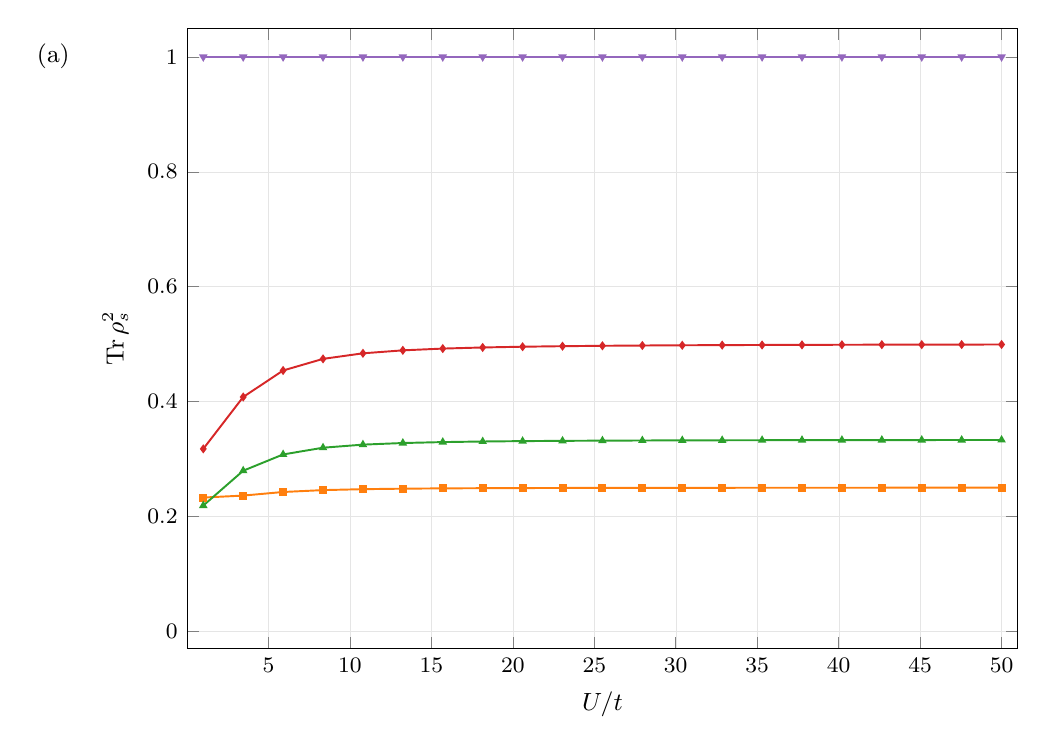
\begin{tikzpicture}
  \begin{axis}[
    width=\columnwidth,
    height=0.78\columnwidth,
    xlabel={$U/t$},
    ylabel={$\mathrm{Tr}\,\rho_s^2$},
    grid=both,
    grid style={line width=.1pt, draw=gray!20},
    tick label style={font=\footnotesize\rmfamily, /pgf/number format/fixed},
    label style={font=\small\rmfamily},
    scaled ticks=false,
    legend style={font=\scriptsize\rmfamily, draw=gray!40, at={(0.5,1.03)}, anchor=south, /tikz/every even column/.append style={column sep=6pt}},
    legend cell align={left},
    legend columns=2,
    ymin=-0.03,
    ymax=1.05,
    xmin=0.02,
    xmax=50.98,
    after end axis/.append code={\node[anchor=east, font=\small\rmfamily] at (axis description cs:-0.13,0.954) {(a)};},
  ]
    \addplot[color=gmeC1, mark=square*, mark size=1.1pt, line width=0.7pt] coordinates {
        (1,0.232704) (3.45,0.236117) (5.9,0.242378) (8.35,0.245651)
        (10.8,0.247275) (13.25,0.248153) (15.7,0.248672) (18.15,0.249001)
        (20.6,0.249222) (23.05,0.249377) (25.5,0.24949) (27.95,0.249575)
        (30.4,0.249641) (32.85,0.249692) (35.3,0.249733) (37.75,0.249767)
        (40.2,0.249794) (42.65,0.249817) (45.1,0.249836) (47.55,0.249853)
        (50,0.249867)
    };
    \addplot[color=gmeC2, mark=triangle*, mark size=1.1pt, line width=0.7pt] coordinates {
        (1,0.218777) (3.45,0.2794) (5.9,0.307755) (8.35,0.319483)
        (10.8,0.324856) (13.25,0.327656) (15.7,0.329278) (18.15,0.330296)
        (20.6,0.330974) (23.05,0.331449) (25.5,0.331794) (27.95,0.332052)
        (30.4,0.33225) (32.85,0.332406) (35.3,0.33253) (37.75,0.332631)
        (40.2,0.332714) (42.65,0.332783) (45.1,0.332841) (47.55,0.332891)
        (50,0.332933)
    };
    \addplot[color=gmeC3, mark=diamond*, mark size=1.1pt, line width=0.7pt] coordinates {
        (1,0.317461) (3.45,0.407797) (5.9,0.453954) (8.35,0.47419)
        (10.8,0.483856) (13.25,0.48904) (15.7,0.492101) (18.15,0.494048)
        (20.6,0.495358) (23.05,0.496281) (25.5,0.496954) (27.95,0.49746)
        (30.4,0.497851) (32.85,0.498157) (35.3,0.498403) (37.75,0.498603)
        (40.2,0.498767) (42.65,0.498904) (45.1,0.49902) (47.55,0.499118)
        (50,0.499202)
    };
    \addplot[color=gmeC4, mark=triangle*, mark size=1.1pt, mark options={rotate=180}, line width=0.7pt] coordinates {
        (1,1) (3.45,1) (5.9,1) (8.35,1)
        (10.8,1) (13.25,1) (15.7,1) (18.15,1)
        (20.6,1) (23.05,1) (25.5,1) (27.95,1)
        (30.4,1) (32.85,1) (35.3,1) (37.75,1)
        (40.2,1) (42.65,1) (45.1,1) (47.55,1)
        (50,1)
    };
  \end{axis}
\end{tikzpicture}
